% -*- latex -*-
% c4.tex
% LabSK 02.06.2022

% Wymagane pola (komentarz):
% Dawid Chmielewski				% Imię Nazwisko

\documentclass[a4paper,11pt]{article}

\usepackage[T1]{polski}
\usepackage[utf8]{inputenc}  			% Kodowanie pliku
\usepackage{pdfpages}

\hoffset=-3.0cm                         % Mniejszy lewy margines
\textwidth=18cm                         % szerzej
\evensidemargin=0pt

\voffset=-3cm                           % Mniejszy górny margines
\textheight=27cm                        % szerzej wzdłuż

\setlength{\parindent}{0pt}             % Paragraf od początku linii
\setlength{\parskip}{\medskipamount}    % Odstęp pomiędzy paragrafami
\raggedbottom                           % bez rozciągania strony

% Dodatkowe komendy
\newcommand\BS{\char`\\}                % \BS == back-slash
\newcommand\TY{\raise.17ex\hbox{$\scriptstyle\mathtt{\sim}$}}   % \TY == większa tylda w \tt

\thispagestyle{empty}			        % bez numeracji stron
\usepackage{enumerate}

\begin{document}
\title{ Sieci komputerowe - sprawozdanie z ćwiczenia 5. }
\author{ Dawid Chmielewski, numer indeksu: 311188 }
\date{24 maja 2022}

\maketitle{Temat ćwiczenia: NAT, serwery i dyski sieciowe}

\section{Założenie dysku w OneDrive}

Dowodem na założenie prywatnego dysku sieciowego jest katalog OneDrive na moim komputerze.

\begin{verbatim}

    PS C:\Users\Dawid> ls One* | ft -a

        Directory: C:\Users\Dawid
    
    Mode        LastWriteTime Length Name
    ----        ------------- ------ ----
    lar-- 01.06.2022    00:38        OneDrive
    
    PS C:\Users\Dawid>

\end{verbatim}

\section{Pobieranie pliku ze swojej strony domowej na volcie}

Do pobierania plików ze swojej strony domowej użyłem programu curl. Pobierany plik można zapisywać pod dowolną nazwą.

\begin{verbatim}

PS C:\Users\Dawid\Desktop> curl http://volt.zet.pw.edu.pl/~chmield2/abc.txt -o abc123.txt
  % Total    % Received % Xferd  Average Speed   Time    Time     Time  Current
                                 Dload  Upload   Total   Spent    Left  Speed
100    16  100    16    0     0    624      0 --:--:-- --:--:-- --:--:--   666
PS C:\Users\Dawid\Desktop> ls ab* | ft -a

    Directory: C:\Users\Dawid\Desktop

Mode        LastWriteTime Length Name
----        ------------- ------ ----
-a--- 01.06.2022    01:03     16 abc123.txt

PS C:\Users\Dawid\Desktop>

\end{verbatim}

\section{Logowanie się bez hasła na stację s1}

Aby móc logować się bez hasła na stację s1, najpierw wygenerowałem parę kluczy i umiesciłem publiczny na githubie, po czym skopiowałem go na stację:

\begin{verbatim}

stud@s1 ~ % curl https://github.com/dawid064.keys >> .ssh/authorized_keys
  % Total    % Received % Xferd  Average Speed   Time    Time     Time  Current
                                 Dload  Upload   Total   Spent    Left  Speed
100   553  100   553    0     0   2962      0 --:--:-- --:--:-- --:--:--  2973
stud@s1 ~ %

\end{verbatim}

To pozwoliło mi na szybkie logowanie bez użycia hasła.
\begin{verbatim}

PS C:\Users\Dawid> ssh stud@10.146.225.1
stud@s1 ~ %

\end{verbatim}

\section{Publikacja kluczy na stronie domowej}

Swój klucz publiczny umieściłem w uprzednio stworzonym katalogu +sshkeys.

\begin{verbatim}

volt% ls WWW/+sshkeys/
id_rsa.pub
volt%

\end{verbatim}

\section{Minimalny schemat sieci}

Przy realizacji ćwiczenia korzystałem z internetu dostępnego w Domu Studenckim Bratniak Politechniki Warszawskiej.

\pagebreak
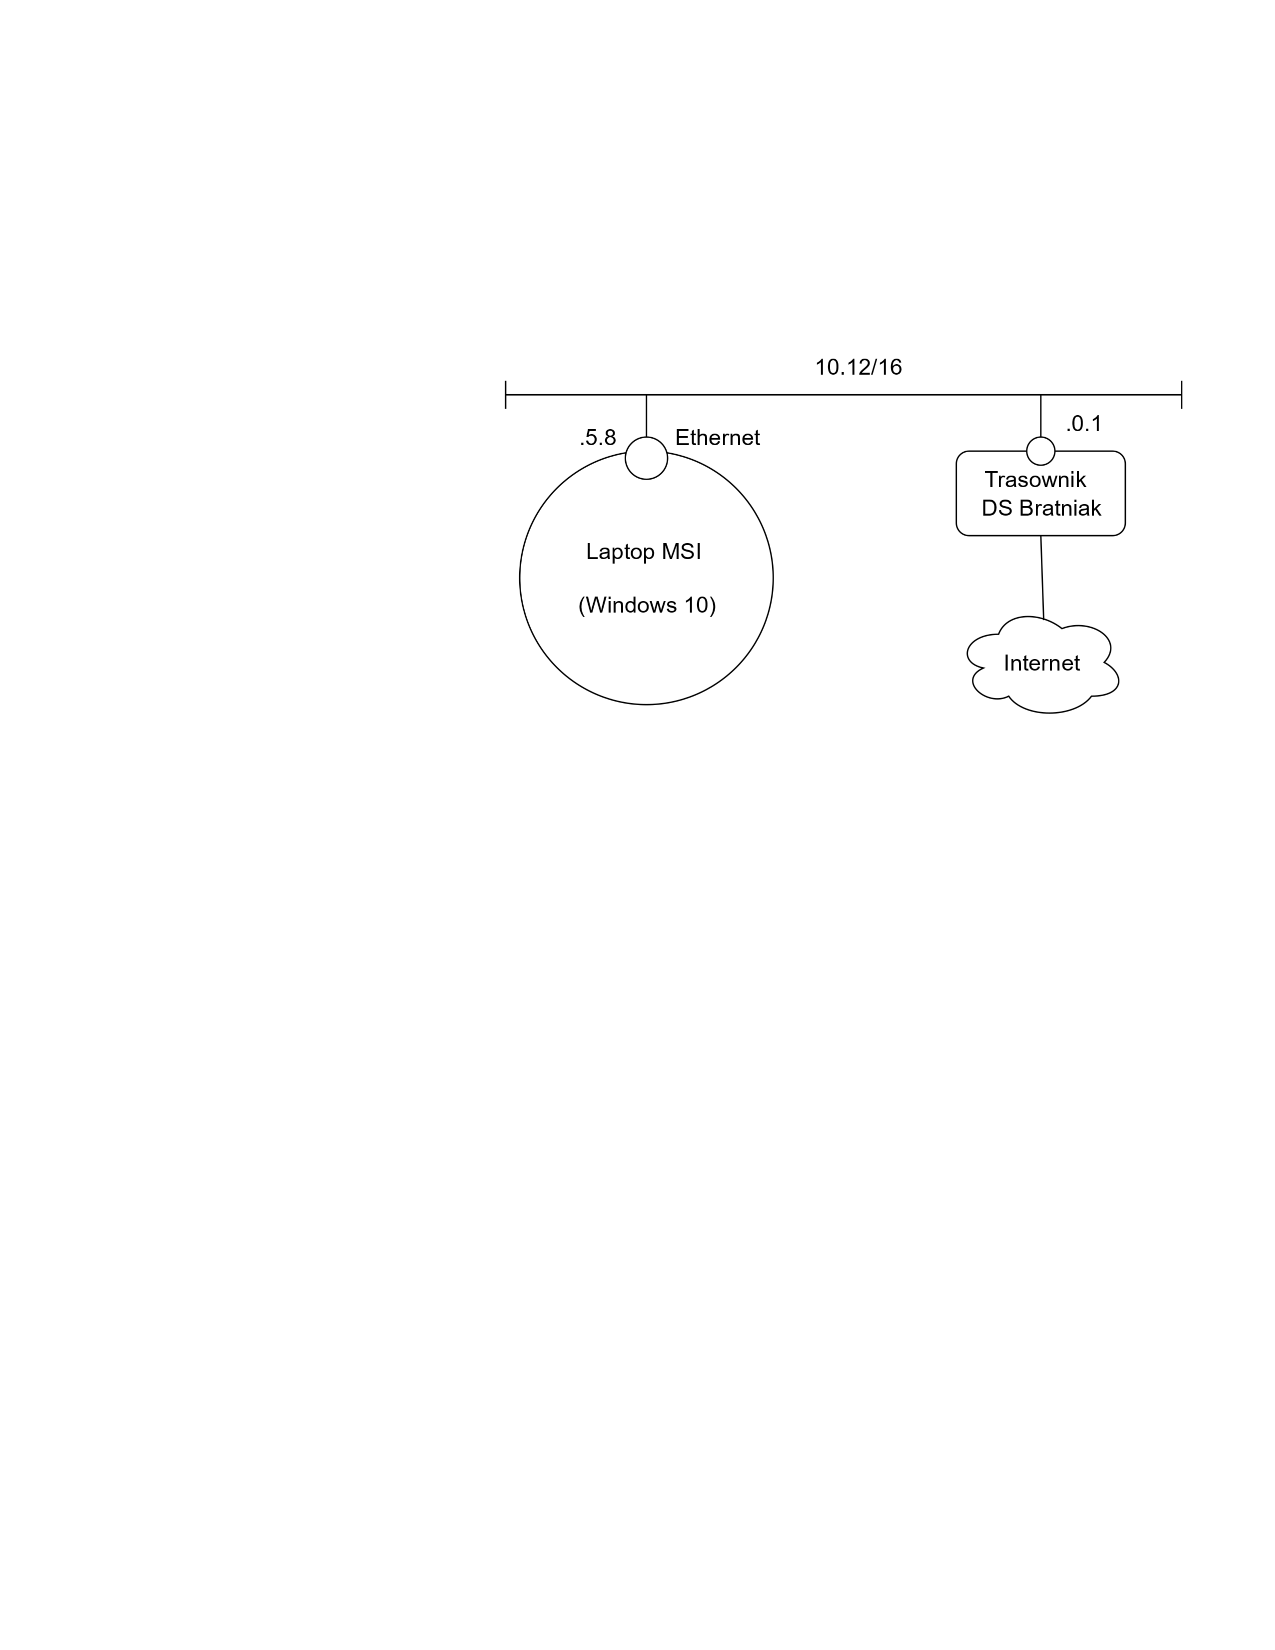
\includepdf[pages=-]{labsk6.pdf}

\end{document}